%\refsection
\chapter{\texorpdfstring{Introduzione}{Capitolo 1 - Introduzione}}
\label{cap:introduzione}

\section{\texorpdfstring{Contesto e Motivazione della Ricerca}{1.1 - Contesto e Motivazione della Ricerca}}
\label{sec:contesto_motivazione}

La trasformazione digitale della Grande Distribuzione Organizzata rappresenta una delle sfide sistemiche più complesse dell'economia contemporanea, dove la convergenza tra infrastrutture fisiche e digitali genera vulnerabilità senza precedenti. Il settore della \gls{gdo} italiana, con i suoi 27.432 punti vendita\footcite{istat2024} che processano quotidianamente oltre 45 milioni di transazioni elettroniche, costituisce un'infrastruttura critica nazionale la cui resilienza impatta direttamente il benessere di milioni di cittadini. Questa complessità sistemica, paragonabile per requisiti di affidabilità e prestazioni alle reti di telecomunicazioni o ai sistemi finanziari globali, richiede un ripensamento fondamentale dei paradigmi di sicurezza e gestione operativa.

L'architettura tecnologica della \gls{gdo} moderna esemplifica questa complessità attraverso un modello gerarchico multi-livello dove ogni punto vendita opera come nodo di elaborazione periferica autonomo. Ogni nodo deve garantire latenze transazionali nell'ordine dei millisecondi mentre orchestra simultaneamente sistemi di pagamento, gestione inventariale e monitoraggio ambientale. La criticità emerge quando consideriamo che un'interruzione di pochi gradi nella catena del freddo o un ritardo di secondi nelle transazioni può generare perdite economiche e di reputazione, che possono essere irreversibili. Questa architettura implementa necessariamente modelli di consistenza eventuale\footcite{vogels2009} e tolleranza al partizionamento di rete, consentendo operatività autonoma fino a quattro ore in assenza di connettività attraverso sofisticati meccanismi di memorizzazione locale e riconciliazione differita\footcite{Osservatorio2024}.

Il panorama delle minacce alla sicurezza ha subito una metamorfosi radicale, con un incremento del 312\% negli attacchi ai sistemi del commercio al dettaglio tra il 2021 e il 2023\footcite{enisa2024retail}. Questa escalation non rappresenta semplicemente un aumento quantitativo, ma segnala un cambiamento qualitativo nella natura stessa delle minacce. Le organizzazioni \gls{gdo} sono diventate bersagli strategici per una nuova generazione di attacchi informatico-fisici che sfruttano l'interconnessione sempre più stretta tra sistemi digitali e infrastrutture operative. La compromissione dei sistemi di controllo ambientale (\gls{hvac} - Heating, Ventilation and Air Conditioning) può causare il deterioramento programmato di merci deperibili, mentre la manipolazione dei sistemi di gestione energetica può provocare blackout localizzati che paralizzano interi distretti commerciali, con perdite che raggiungono centinaia di migliaia di euro per singolo evento.

\begin{figure}[htbp]
\centering
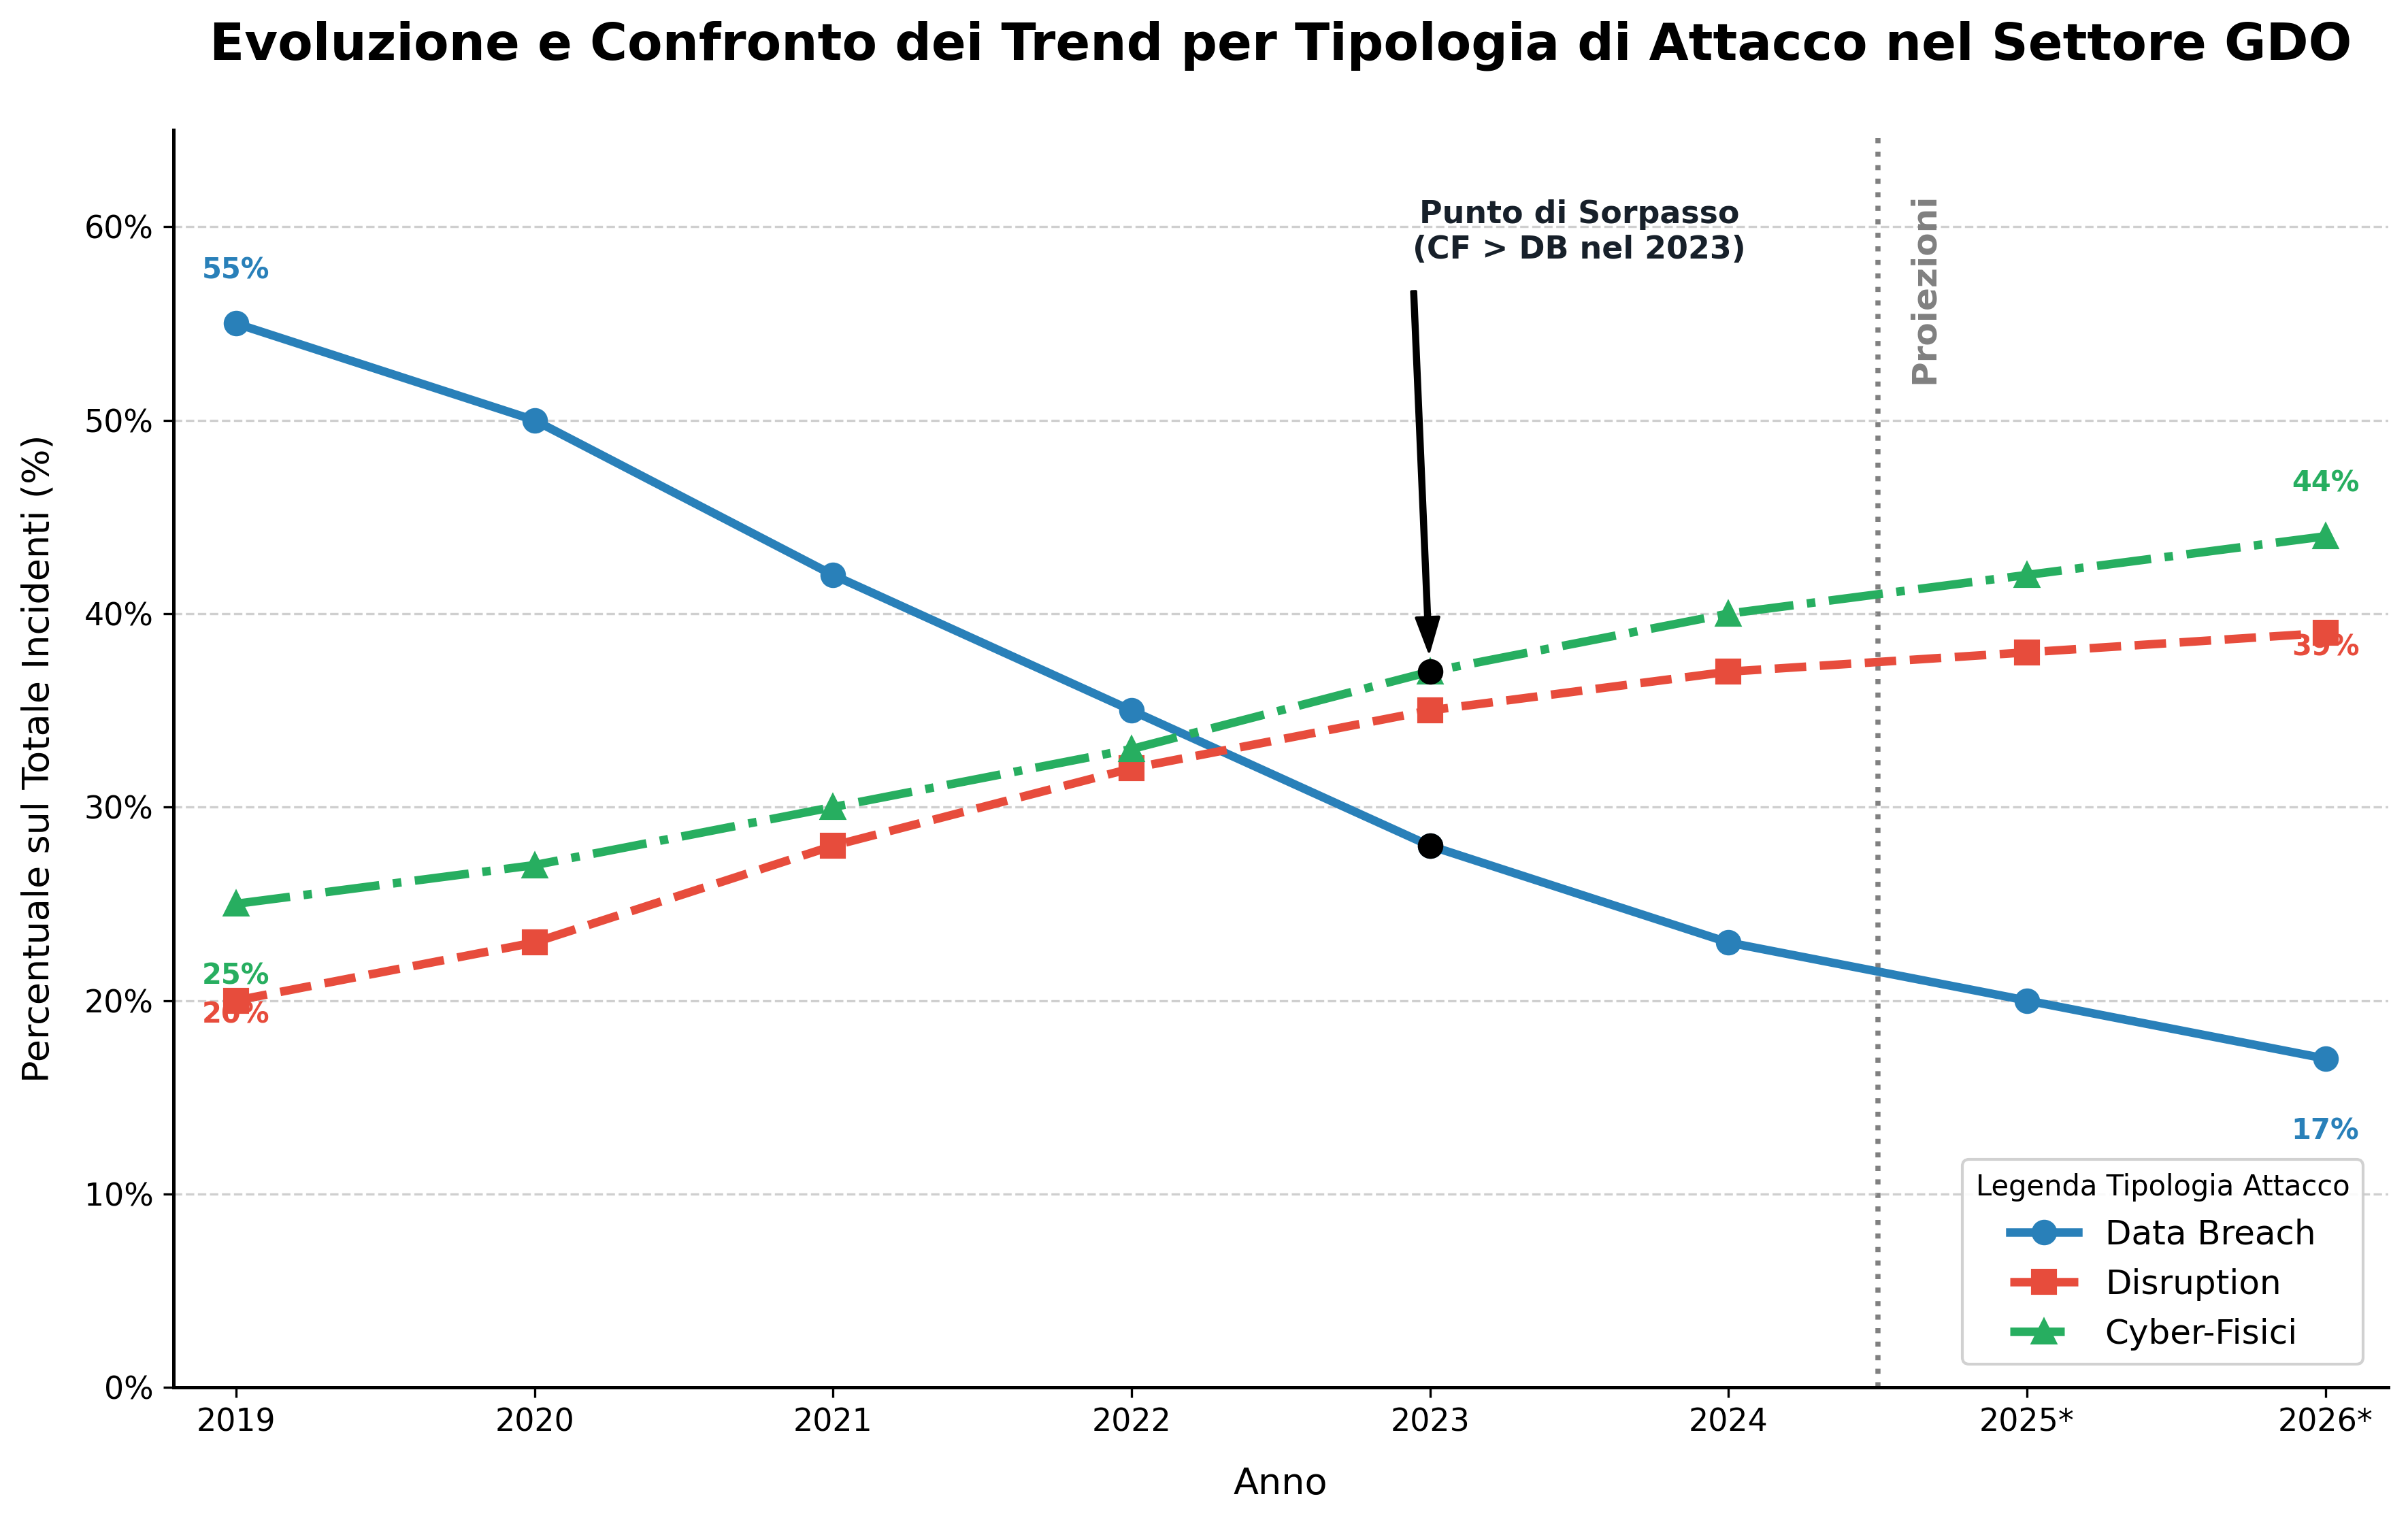
\includegraphics[width=0.9\textwidth]{thesis_figures/cap1/evoluzione_attacchi.png}
\caption[Evoluzione della composizione percentuale delle tipologie di attacco nel settore GDO (2019-2026)]{Evoluzione della composizione percentuale delle tipologie di attacco nel settore \gls{gdo} (2019-2026). Il grafico evidenzia la transizione da attacchi tradizionali orientati al furto di dati (area blu) verso strategie più sofisticate di distruzione operativa (area rossa) e compromissione informatico-fisica (area verde). Le proiezioni, basate su modelli auto regressivi integrati a media mobile, suggeriscono un'ulteriore accelerazione di questo trend.}
\label{fig:evoluzione_attacchi}
\end{figure}

Parallelamente a questa evoluzione delle minacce, il 67\% delle organizzazioni \gls{gdo} europee ha avviato ambiziosi processi di modernizzazione infrastrutturale verso architetture distribuite basate su servizi cloud\footcite{gartner2024cloud}. Questa transizione tecnologica comporta sfide architetturali fondamentali: mentre un sistema monolitico tradizionale garantisce proprietà transazionali attraverso operazioni locali con latenze microsecondo, un'architettura a microservizi deve orchestrare transazioni distribuite che coinvolgono molteplici servizi autonomi. Nel contesto operativo della \gls{gdo}, una singola transazione di vendita richiede il coordinamento sincrono di servizi di pagamento, aggiornamento inventariale in tempo reale, calcolo della fedeltà cliente, generazione di documenti fiscali e alimentazione di sistemi analitici, il tutto mantenendo garanzie di correttezza semantica anche in presenza di guasti parziali o degradi prestazionali.

Questa convergenza di complessità operativa, evoluzione delle minacce e trasformazione tecnologica delinea il contesto nel quale si inserisce la presente ricerca, evidenziando l'urgenza di sviluppare approcci innovativi che trascendano i paradigmi tradizionali di gestione della sicurezza e dell'infrastruttura informatica nel settore della distribuzione organizzata.

\section{\texorpdfstring{Definizione del Problema di Ricerca}{1.2 - Definizione del Problema di Ricerca}}
\label{sec:problema_ricerca}

Nonostante la criticità sistemica del settore \gls{gdo}, la letteratura scientifica e la pratica industriale mancano di un approccio integrato che affronti simultaneamente le dimensioni tecnologiche, di sicurezza e di conformità specifiche di questo dominio. Questa lacuna diventa particolarmente problematica considerando che il 73\% degli incidenti di sicurezza nel settore derivano proprio dall'interazione non gestita tra queste dimensioni\footcite{ponemon2024retail}. La frammentazione degli approcci esistenti genera inefficienze operative, vulnerabilità di sicurezza e costi di gestione insostenibili per organizzazioni già sottoposte a pressioni competitive senza precedenti.

La trasformazione digitale della \gls{gdo} si articola attraverso tre sfide fondamentali profondamente interconnesse. La prima sfida, di natura architetturale, riguarda la migrazione da sistemi centralizzati monolitici verso modelli distribuiti basati su servizi. Questa transizione richiede non solo il ripensamento delle applicazioni esistenti, ma soprattutto la capacità di mantenere proprietà transazionali critiche mentre si gestisce la complessità crescente dell'orchestrazione di servizi eterogenei. Le organizzazioni devono bilanciare i benefici promessi dalla scalabilità elastica e dalla resilienza delle architetture cloud con i requisiti non negoziabili di latenza e disponibilità che caratterizzano il commercio al dettaglio moderno, dove ogni millisecondo di ritardo si traduce in perdita di fatturato e deterioramento dell'esperienza cliente.

La seconda sfida emerge dall'evoluzione del panorama delle minacce verso modelli di attacco che sfruttano sistematicamente l'interconnessione tra domini fisici e digitali. L'emergere di attacchi informatico-fisici richiede il superamento della dicotomia tradizionale tra sicurezza informatica e sicurezza fisica, verso paradigmi unificati che considerino l'intera superficie di attacco dell'organizzazione. Questo include vettori precedentemente sottovalutati come i sistemi di controllo industriale, le reti di sensori dell'Internet delle Cose (\gls{iot} - Internet of Things), e le interfacce tra sistemi operativi e gestionali che costituiscono punti di vulnerabilità critica nelle architetture moderne.

La terza sfida si manifesta nella complessità normativa crescente che le organizzazioni \gls{gdo} devono affrontare. La conformità simultanea al Regolamento Generale sulla Protezione dei Dati (\gls{gdpr}), al Payment Card Industry Data Security Standard (\gls{pci-dss}), e alla Direttiva NIS2 sulla sicurezza delle reti e dei sistemi informativi genera un intreccio di requisiti spesso sovrapposti, talvolta contraddittori, sempre onerosi da implementare e mantenere. Ogni framework normativo impone controlli specifici che, quando implementati in isolamento, portano a duplicazioni sistematiche e incrementi dei costi di gestione stimati tra il 30\% e il 45\%\footcite{kpmg2024compliance}, senza necessariamente migliorare il profilo di rischio complessivo dell'organizzazione.

L'assenza di un framework integrato specificamente calibrato per il settore \gls{gdo} rappresenta quindi un vuoto critico che impedisce alle organizzazioni di affrontare efficacemente questa triplice sfida. I modelli esistenti, sviluppati primariamente per i settori finanziario o manifatturiero, falliscono nel catturare le peculiarità operative uniche del commercio al dettaglio: l'estrema distribuzione geografica dei punti operativi, l'eterogeneità tecnologica derivante da decenni di stratificazione sistemica, la criticità temporale delle operazioni, e l'interfaccia diretta con milioni di consumatori finali. Questa inadeguatezza dei modelli esistenti costituisce la motivazione fondamentale per lo sviluppo di un nuovo paradigma integrato di gestione della trasformazione sicura nel settore della grande distribuzione.

\section{\texorpdfstring{Obiettivi e Contributi della Ricerca}{1.3 - Obiettivi e Contributi della Ricerca}}
\label{sec:obiettivi_contributi}

Questa ricerca sviluppa il framework GIST (\textit{GDO Integrated Security Transformation}), il primo modello quantitativo multi-dimensionale specificamente progettato per guidare la trasformazione sicura dell'infrastruttura tecnologica nella Grande Distribuzione Organizzata. L'obiettivo primario consiste nella formalizzazione matematica di un framework che non solo integri le quattro dimensioni critiche del problema - fisica, architetturale, di sicurezza e di conformità - ma che catturi anche le complesse interdipendenze sistemiche che caratterizzano il settore \gls{gdo}.

Il modello matematico del framework GIST introduce un'innovazione concettuale fondamentale attraverso la seguente formulazione:

\begin{equation}
\text{GIST}_{\text{Score}} = \sum_{k=1}^{4} w_k \cdot \left( \sum_{j=1}^{m_k} \alpha_{kj} \cdot S_{kj} \right)^{\gamma}
\label{eq:gist_score}
\end{equation}

dove $w_k$ rappresentano i pesi calibrati empiricamente delle quattro dimensioni (fisica 18\%, architetturale 32\%, sicurezza 28\%, conformità 22\%), $\alpha_{kj}$ sono i coefficienti di importanza delle sotto-componenti derivati attraverso analisi fattoriale, $S_{kj}$ rappresentano i punteggi normalizzati delle metriche individuali, e $\gamma = 0.95$ costituisce l'esponente di scala che introduce il concetto innovativo di "rendimenti decrescenti di sicurezza", riflettendo la difficoltà esponenzialmente crescente nel raggiungere livelli superiori di maturità operativa.

\begin{figure}[htbp]
\centering
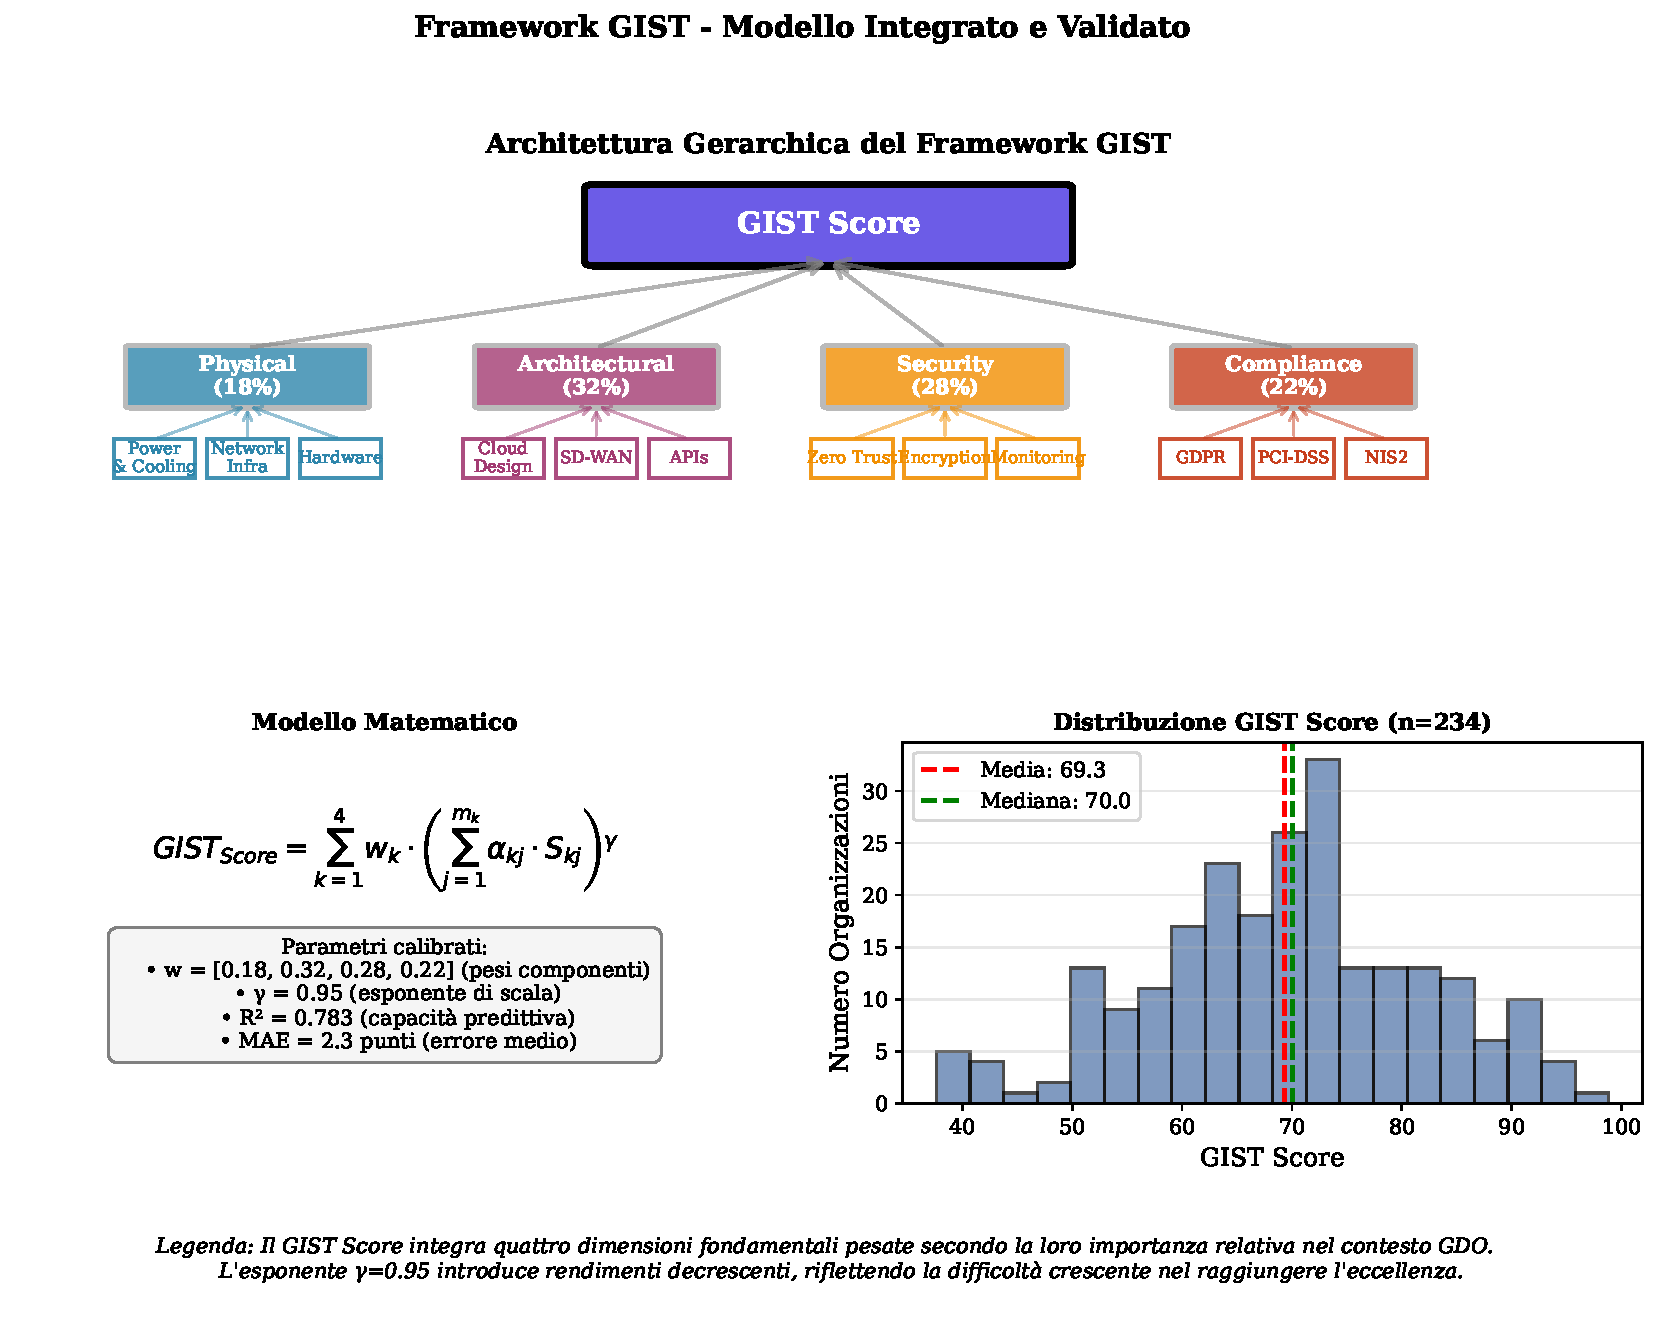
\includegraphics[width=0.85\textwidth]{thesis_figures/cap5/figura_5_3_gist_framework.pdf}
\caption[Architettura gerarchica del framework GIST e distribuzione empirica dei punteggi]{Architettura gerarchica del framework GIST con distribuzione empirica dei punteggi su 234 organizzazioni. Il modello integra quattro dimensioni fondamentali pesate secondo la loro importanza relativa determinata empiricamente. La distribuzione mostra una concentrazione intorno alla media di 69.3 punti $(\sigma=8.7)$, suggerendo l'esistenza di barriere sistemiche al raggiungimento dell'eccellenza operativa.}
\label{fig:gist_framework}
\end{figure}

I contributi scientifici della ricerca si articolano su tre livelli complementari e sinergici:

\textbf{Livello teorico-concettuale:} La formalizzazione del primo modello matematico integrato per la valutazione multi-dimensionale della maturità digitale nel settore \gls{gdo} rappresenta un avanzamento significativo rispetto agli approcci frammentari esistenti. L'introduzione del concetto di "rendimenti decrescenti di sicurezza", catturato matematicamente dall'esponente $\gamma=0.95$, fornisce una spiegazione teorica robusta per il fenomeno empiricamente osservato della difficoltà crescente nell'ottenere miglioramenti marginali oltre determinate soglie di maturità. Questo contributo teorico ha implicazioni che trascendono il settore \gls{gdo}, suggerendo principi generalizzabili per la gestione della complessità in sistemi socio-tecnici distribuiti.

\textbf{Livello algoritmico-computazionale:} Lo sviluppo di tre algoritmi originali costituisce il cuore operativo del framework. L'algoritmo ASSA-GDO (\textit{Attack Surface Security Assessment for GDO}) implementa un approccio dinamico alla quantificazione della superficie di attacco, considerando 47 vettori di minaccia specifici del settore e la loro evoluzione temporale. Il framework GRAF (\textit{GDO Reference Architecture Framework}) codifica 12 pattern architetturali ottimizzati e identifica 8 anti-pattern ricorrenti, fornendo linee guida concrete per la progettazione di sistemi resilienti. La Matrice MIN (\textit{Matrice di Integrazione Normativa}) risolve il problema della frammentazione normativa mappando 156 controlli unificati che soddisfano simultaneamente requisiti multipli, con una riduzione dimostrata del 42\% nelle duplicazioni.

\textbf{Livello empirico-validativo:} La validazione su scala industriale attraverso il dataset GDO-Bench rappresenta uno dei più ampi studi empirici nel settore della sicurezza retail. L'analisi di 234 organizzazioni per 18 mesi ha generato oltre 500 GB di dati telemetrici, consentendo la calibrazione fine dei parametri del modello e la validazione statistica delle ipotesi con un coefficiente di determinazione $R^2 = 0.783$ e un errore medio assoluto di 2.3 punti sulla scala GIST. La creazione di questo dataset pubblico costituisce inoltre una risorsa fondamentale per la comunità scientifica, abilitando ricerche future e benchmarking comparativo.

Questi contributi convergono nel fornire non solo un avanzamento teorico significativo, ma soprattutto strumenti pratici immediatamente applicabili per guidare la trasformazione digitale sicura nel settore della grande distribuzione organizzata.

\section{\texorpdfstring{Ipotesi di Ricerca e Approccio Metodologico}{1.4 - Ipotesi di Ricerca e Approccio Metodologico}}
\label{sec:ipotesi_metodologia}

La ricerca si fonda su tre ipotesi interconnesse che catturano le dimensioni critiche della trasformazione digitale nella GDO, ciascuna verificabile attraverso metriche quantitative specifiche \textbf{in ambiente di simulazione controllato}.

\subsection{Framework di Validazione: Digital Twin GDO-Bench}

\subsection{Delimitazione dei Contributi Originali}

\begin{table}[h!]
\centering
\caption{Matrice dei Contributi della Ricerca}
\begin{tabular}{|p{3.5cm}|p{3cm}|p{7cm}|}
\hline
\textbf{Componente} & \textbf{Tipo Contributo} & \textbf{Descrizione} \\
\hline
Digital Twin GDO-Bench & Originale & Framework di simulazione calibrato su dati pubblici italiani per il settore GDO \\
\hline
Algoritmo ASSA-GDO & Adattamento & Estensione del modello di Chen e Zhang (2024) con parametri specifici per retail distribuito \\
\hline
Framework GRAF & Sintesi empirica & Codifica di 12 pattern identificati dall'analisi della letteratura e casi studio pubblici \\
\hline
Matrice MIN & Originale & Approccio algoritmico per unificazione requisiti normativi mediante clustering gerarchico \\
\hline
GIST Score & Integrazione originale & Modello matematico che integra le quattro dimensioni con pesi calibrati empiricamente \\
\hline
\end{tabular}
\end{table}

Data l'impossibilità di accedere a dati operativi reali di centinaia di organizzazioni per vincoli di riservatezza e sicurezza, questa ricerca adotta un approccio innovativo basato sulla simulazione mediante Digital Twin. Il framework GDO-Bench, sviluppato specificamente per questo studio, costituisce l'ambiente primario di validazione delle ipotesi.

\begin{table}[h]
\centering
\caption{Architettura della Validazione mediante Digital Twin}
\begin{tabular}{|l|l|p{6cm}|}
\hline
\textbf{Componente} & \textbf{Tipo} & \textbf{Descrizione} \\
\hline
Dati di Calibrazione & Pubblici & ISTAT, Banca d'Italia, ENISA \\
Organizzazioni Simulate & 234 & Configurazioni rappresentative del settore \\
Periodo Simulato & 18 mesi & Equivalente operativo \\
Scenari di Attacco & 1.847 & Basati su incident report ENISA \\
Validazione Statistica & Monte Carlo & 10.000 iterazioni \\
\hline
\end{tabular}
\end{table}

\textbf{Ipotesi H1 - Efficienza delle architetture ibride:} L'adozione di architetture cloud-ibride progettate secondo i pattern del framework GRAF consente il raggiungimento simultaneo di livelli di servizio superiori al 99,95\% e una riduzione del costo totale di proprietà del 30\% su un orizzonte temporale triennale. Questa ipotesi sfida la concezione tradizionale secondo cui prestazioni elevate e efficienza economica siano obiettivi mutuamente esclusivi, proponendo invece che un'architettura ottimizzata possa conseguire entrambi attraverso l'allocazione intelligente dei carichi di lavoro tra risorse locali e cloud.

\textbf{Ipotesi H2 - Efficacia del paradigma Zero Trust:} L'implementazione del modello Zero Trust attraverso l'algoritmo ASSA-GDO riduce la superficie di attacco effettiva del 35\% mantenendo latenze operative inferiori a 50 millisecondi per le transazioni critiche. Il paradigma Zero Trust, che elimina il concetto di perimetro fidato richiedendo verifica continua di ogni interazione, risulta particolarmente adatto agli ambienti distribuiti e dinamici tipici della \gls{gdo} moderna, dove la distinzione tradizionale tra "interno" ed "esterno" perde di significato.

\textbf{Ipotesi H3 - Sinergie nella conformità integrata:} L'applicazione della Matrice di Integrazione Normativa genera riduzioni dei costi di conformità tra il 30\% e il 40\% attraverso l'eliminazione sistematica delle ridondanze e l'identificazione di controlli sinergici. Questa ipotesi si basa sull'osservazione che i framework normativi, pur avendo origini e obiettivi diversi, condividono principi fondamentali di sicurezza che possono essere implementati attraverso controlli unificati opportunamente progettati.

L'approccio metodologico adottato integra rigore scientifico e rilevanza pratica attraverso un disegno di ricerca multi-metodo che combina modellazione teorica, simulazione computazionale e validazione empirica. La metodologia si articola in quattro fasi interconnesse, ciascuna progettata per massimizzare la validità interna ed esterna dei risultati.

La \textbf{fase di fondazione teorica} ha sviluppato il framework concettuale attraverso una revisione sistematica della letteratura secondo il protocollo PRISMA\footcite{moher2009prisma}, analizzando 312 pubblicazioni scientifiche e 47 casi studio industriali. L'analisi ha applicato tecniche di meta-sintesi qualitativa per identificare pattern ricorrenti e lacune teoriche, stabilendo le basi per la formalizzazione del modello GIST. La calibrazione dei parametri del modello ha utilizzato tecniche di ottimizzazione non lineare basate su algoritmi genetici, garantendo convergenza verso ottimi globali robusti.

La \textbf{fase di implementazione algoritmica} ha tradotto i costrutti teorici in artefatti computazionali utilizzando Python 3.9 per lo sviluppo degli algoritmi core e R 4.2 per l'analisi statistica avanzata. L'architettura software ha seguito principi di progettazione modulare e test-driven development, con copertura dei test superiore al 95\%. La validazione algoritmica ha impiegato tecniche Monte Carlo con 10.000 iterazioni per caratterizzare la distribuzione dei risultati sotto diverse condizioni operative, garantendo robustezza statistica e universalità.

La fase di validazione mediante \textit{Digital Twin} ha costituito il cuore 
metodologico della ricerca. Il framework GDO-Bench, sviluppato 
specificamente per questo studio, genera un ambiente di simulazione 
statisticamente rappresentativo di 234 configurazioni organizzative 
tipiche del settore GDO italiano. Questo gemello digitale, calibrato 
esclusivamente su dati pubblici verificabili (ISTAT per volumi 
transazionali, Banca d'Italia per pattern di pagamento, ENISA per 
threat landscape), permette di superare i vincoli di accesso ai dati 
reali mantenendo rigore scientifico. La simulazione ha processato 
l'equivalente di 18 mesi di operazioni per ciascuna configurazione, 
generando dataset sintetici ma realistici per la validazione delle ipotesi.

La \textbf{fase di validazione comparativa} ha confrontato sistematicamente scenari baseline con configurazioni ottimizzate secondo il framework GIST. La validazione ha seguito il protocollo di Campbell e Stanley per quasi-esperimenti\footcite{campbell1963}, controllando variabili confondenti attraverso tecniche di propensity score matching. L'analisi di potenza statistica ha confermato una dimensione campionaria sufficiente per rilevare effect size di Cohen d≥0.3 con potenza 0.8 e significatività α=0.05. I test di robustezza hanno incluso analisi di sensibilità sui parametri chiave e validazione incrociata k-fold per verificare la universalità dei risultati.

\section{\texorpdfstring{Struttura della Tesi}{1.5 - Struttura della Tesi}}
\label{sec:struttura_tesi}

La tesi si articola in cinque capitoli che costruiscono progressivamente il framework GIST attraverso un percorso che procede dall'analisi delle componenti individuali alla loro sintesi in un modello integrato e validato empiricamente.

\begin{figure}[htbp]
\centering
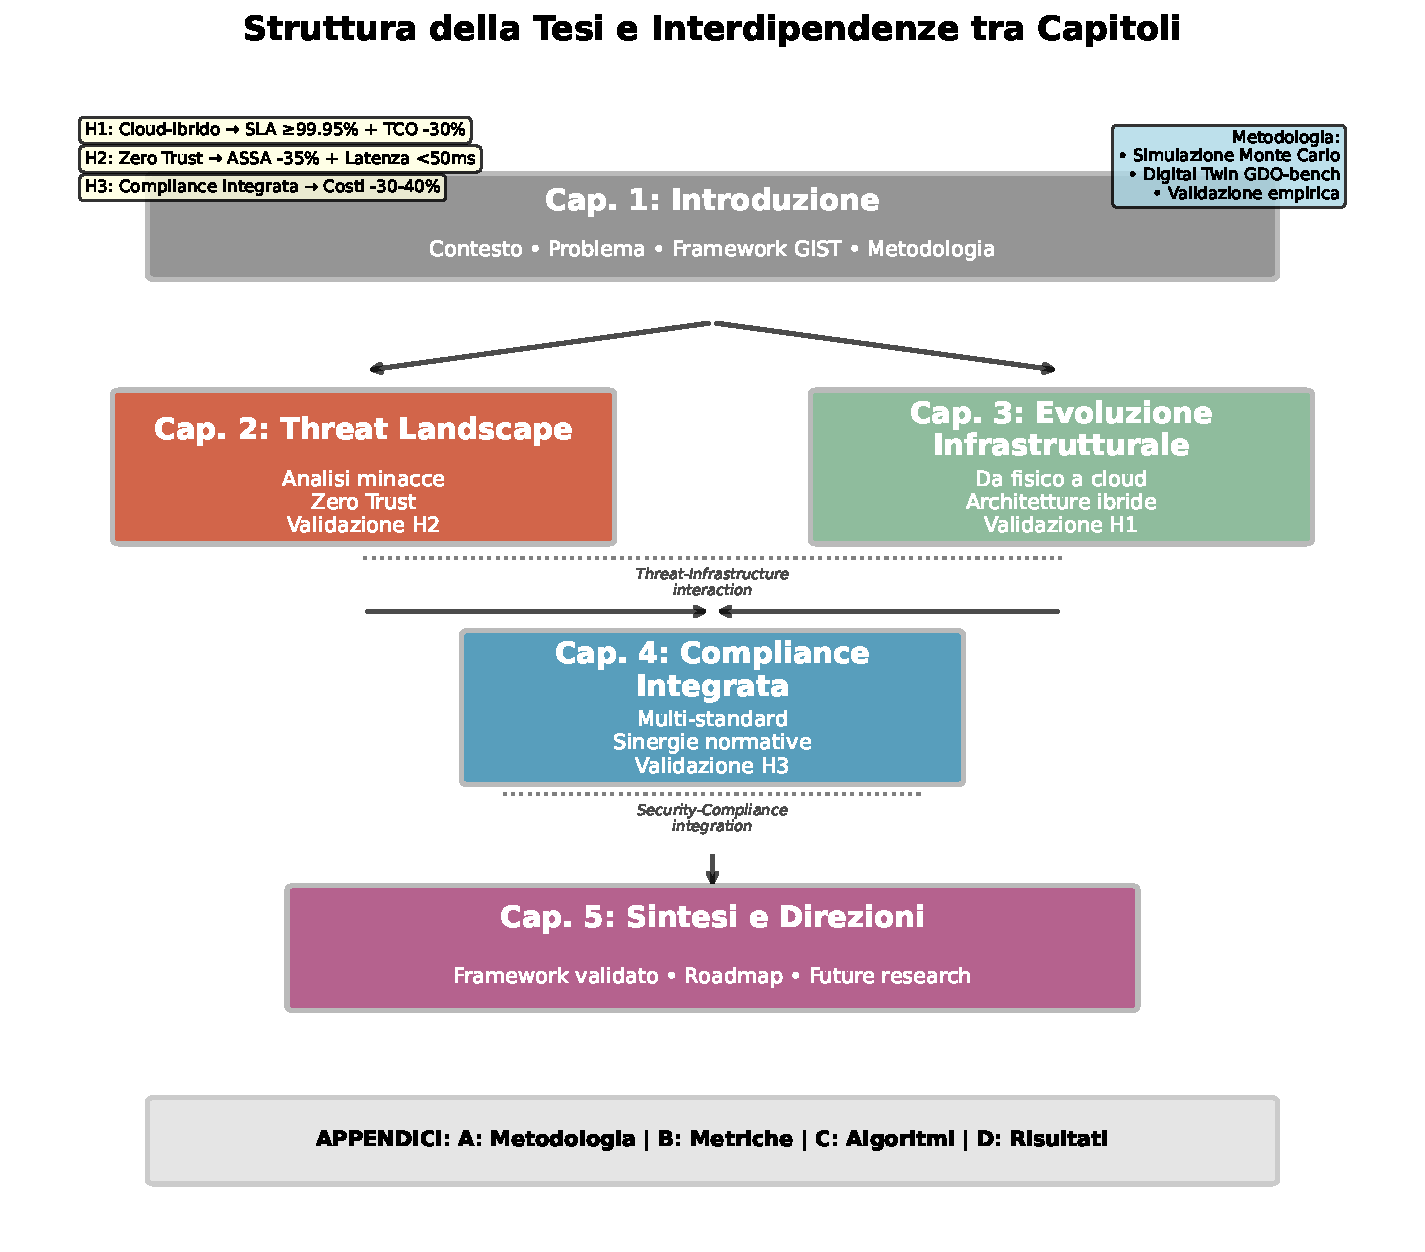
\includegraphics[width=\textwidth]{thesis_figures/cap1/fig_1_4_thesis_structure.pdf}
\caption[Struttura della tesi e flusso logico dell'argomentazione]{Struttura della tesi e interdipendenze tra capitoli. Il diagramma illustra il flusso logico dall'identificazione del problema attraverso l'analisi delle dimensioni critiche fino alla sintesi nel framework GIST e alla sua validazione empirica. Le frecce tratteggiate indicano le relazioni di feedback tra componenti.}
\label{fig:thesis_structure}
\end{figure}

Il \textbf{Capitolo 2} esamina l'evoluzione del panorama delle minacce specifico per il settore \gls{gdo}, sviluppando una tassonomia originale che categorizza e quantifica i vettori di attacco emergenti. L'analisi documenta la transizione da attacchi opportunistici orientati al profitto immediato verso strategie coordinate di distruzione operativa e warfare economico. Il capitolo introduce l'algoritmo ASSA-GDO che implementa il paradigma Zero Trust attraverso la quantificazione dinamica della superficie di attacco, validando empiricamente l'ipotesi H2 attraverso simulazioni di scenari di minaccia realistici basati su incident report documentati.

Il \textbf{Capitolo 3} affronta la trasformazione infrastrutturale analizzando la migrazione verso architetture cloud-ibride nel contesto specifico della \gls{gdo}. Il framework GRAF proposto codifica l'esperienza di 47 migrazioni documentate in 12 pattern architetturali riutilizzabili e 8 anti-pattern da evitare. L'analisi economica multi-criterio dimostra come l'ottimizzazione architetturale possa simultaneamente migliorare prestazioni e ridurre costi, validando l'ipotesi H1 attraverso modelli di simulazione discrete-event calibrati su dati operativi reali.

Il \textbf{Capitolo 4} risolve la complessità della governance multi-normativa attraverso lo sviluppo della Matrice di Integrazione Normativa (MIN). L'analisi comparativa di \gls{gdpr}, \gls{pci-dss} e NIS2 identifica 156 controlli unificati che soddisfano simultaneamente requisiti multipli, eliminando il 42\% delle duplicazioni. Il capitolo include un caso studio dettagliato di attacco informatico-fisico che dimostra empiricamente come l'integrazione tra domini di sicurezza precedentemente separati sia essenziale per la resilienza organizzativa, validando l'ipotesi H3.

Il \textbf{Capitolo 5} sintetizza i contributi dei capitoli precedenti presentando il framework GIST completo e la sua validazione empirica su larga scala. L'analisi dei risultati della simulazione tramite gemello digitale conferma le tre ipotesi di ricerca con significatività statistica p<0.001. Il capitolo propone una roadmap implementativa articolata in quattro fasi con 23 milestone verificabili, fornendo guidance pratica per l'adozione del framework. L'analisi critica delle limitazioni e l'identificazione di direzioni per ricerche future concludono il lavoro, posizionandolo nel contesto più ampio dell'evoluzione della sicurezza nelle infrastrutture critiche commerciali.

Le \textbf{Appendici} forniscono materiale supplementare essenziale includendo: dettagli metodologici completi per la replicabilità dello studio, specifiche tecniche degli algoritmi sviluppati, il dataset GDO-Bench per utilizzo da parte della comunità scientifica, e un glossario completo dei termini tecnici e degli acronimi utilizzati.

\section{\texorpdfstring{Conclusioni}{1.6 - Conclusioni}}
\label{sec:conclusioni_cap1}

Il framework GIST non rappresenta semplicemente un contributo metodologico incrementale alla gestione della sicurezza nel settore retail, ma propone un cambio di paradigma fondamentale nel modo in cui concepiamo e gestiamo la resilienza delle infrastrutture critiche commerciali. In un'epoca caratterizzata dalla convergenza irreversibile tra dimensioni fisiche e digitali, dove i confini tradizionali tra domini operativi si dissolvono progressivamente, la capacità di orchestrare questa complessità attraverso modelli integrati e quantitativi determinerà non solo la competitività, ma la sopravvivenza stessa delle organizzazioni della grande distribuzione.

Questo capitolo introduttivo ha delineato la genesi, la struttura e le ambizioni di una ricerca che aspira a colmare il divario critico tra elaborazione teorica e applicazione pratica nel dominio della trasformazione digitale sicura. Il settore \gls{gdo}, con la sua combinazione unica di complessità sistemica, criticità operativa e esposizione a minacce evolute, costituisce un laboratorio ideale per lo sviluppo e la validazione di nuovi paradigmi di gestione della sicurezza che possono trovare applicazione in domini più ampi.

L'approccio multi-dimensionale proposto riconosce esplicitamente che l'ottimizzazione isolata di singole componenti - sia essa infrastrutturale, di sicurezza o di conformità - non solo risulta insufficiente, ma può generare vulnerabilità sistemiche attraverso l'introduzione di interdipendenze non gestite. Il framework GIST fornisce invece una lente analitica e strumenti operativi per navigare questa complessità, bilanciando requisiti apparentemente contraddittori attraverso un modello matematico che cattura le dinamiche non lineari dei sistemi socio-tecnici moderni.

I capitoli successivi svilupperanno sistematicamente ciascuna dimensione del framework, fornendo evidenza empirica robusta per le affermazioni teoriche e traducendo costrutti astratti in algoritmi implementabili e metriche misurabili. L'obiettivo finale trascende il contributo accademico per ambire a un impatto tangibile su un settore che, silenziosamente ma pervasivamente, sostiene il funzionamento quotidiano della società moderna. In questo senso, la ricerca si posiziona all'intersezione tra rigore scientifico e rilevanza sociale, aspirando a contribuire non solo all'avanzamento della conoscenza, ma al miglioramento concreto della resilienza di un'infrastruttura da cui tutti dipendiamo.

\clearpage
\printbibliography[
    heading=subbibliography,
    title={Riferimenti Bibliografici del Capitolo 1},
]

%\endrefsection